\chapter{Implementasi dan Pengujian}
\label{chap:implementasi&pengujian}

% Pada bab ini akan dijelaskan mengenai implementasi perangkat lunak, serta pengujian perangkat
% lunak. Implementasi perangkat lunak berisi penjelasan lingkungan pengembangan perangkat lunak dan hasil
% implementasi. Sedangkan pengujian perangkat lunak berisi hasil pengujian fungsional dan eksperimental
% terhadap perangkat lunak yang telah dibangun.

Pada bab ini akan dijelaskan mengenai lingkungan pengembangan perangkat lunak dan hasil
implementasi.

\section{Lingkungan Implementasi}
\label{lingkungan_implementasi}
Implementasi perangkat lunak ini dilakukan di komputer penulis dengan spesifikasi berikut:
\begin{enumerate}
    \item \textit{Processor}: Intel Core i5-10300H
    \item \textit{Random Access Memory(RAM)}: 16 GB DDR4
    \item Sistem Operasi: Windows 10
    \item Versi Java: 15.0.1
    \item Versi JavaFX: 8.0.202
    \item Versi Netbeans: 12.1
    \item Versi Scenebuilder: 11.0.0
\end{enumerate}

\section{Hasil Implementasi}
Hasil implementasi berupa aplikasi \textit{screensaver}, dimana aplikasi tersebut akan dijalankan secara otomatis setelah komputer tidak digunakan selama beberapa saat. Gambar \ref{fig:5_hasil} merupakan tampilan dari aplikasi \textit{screensaver}.

\begin{figure}[H]
	\centering
	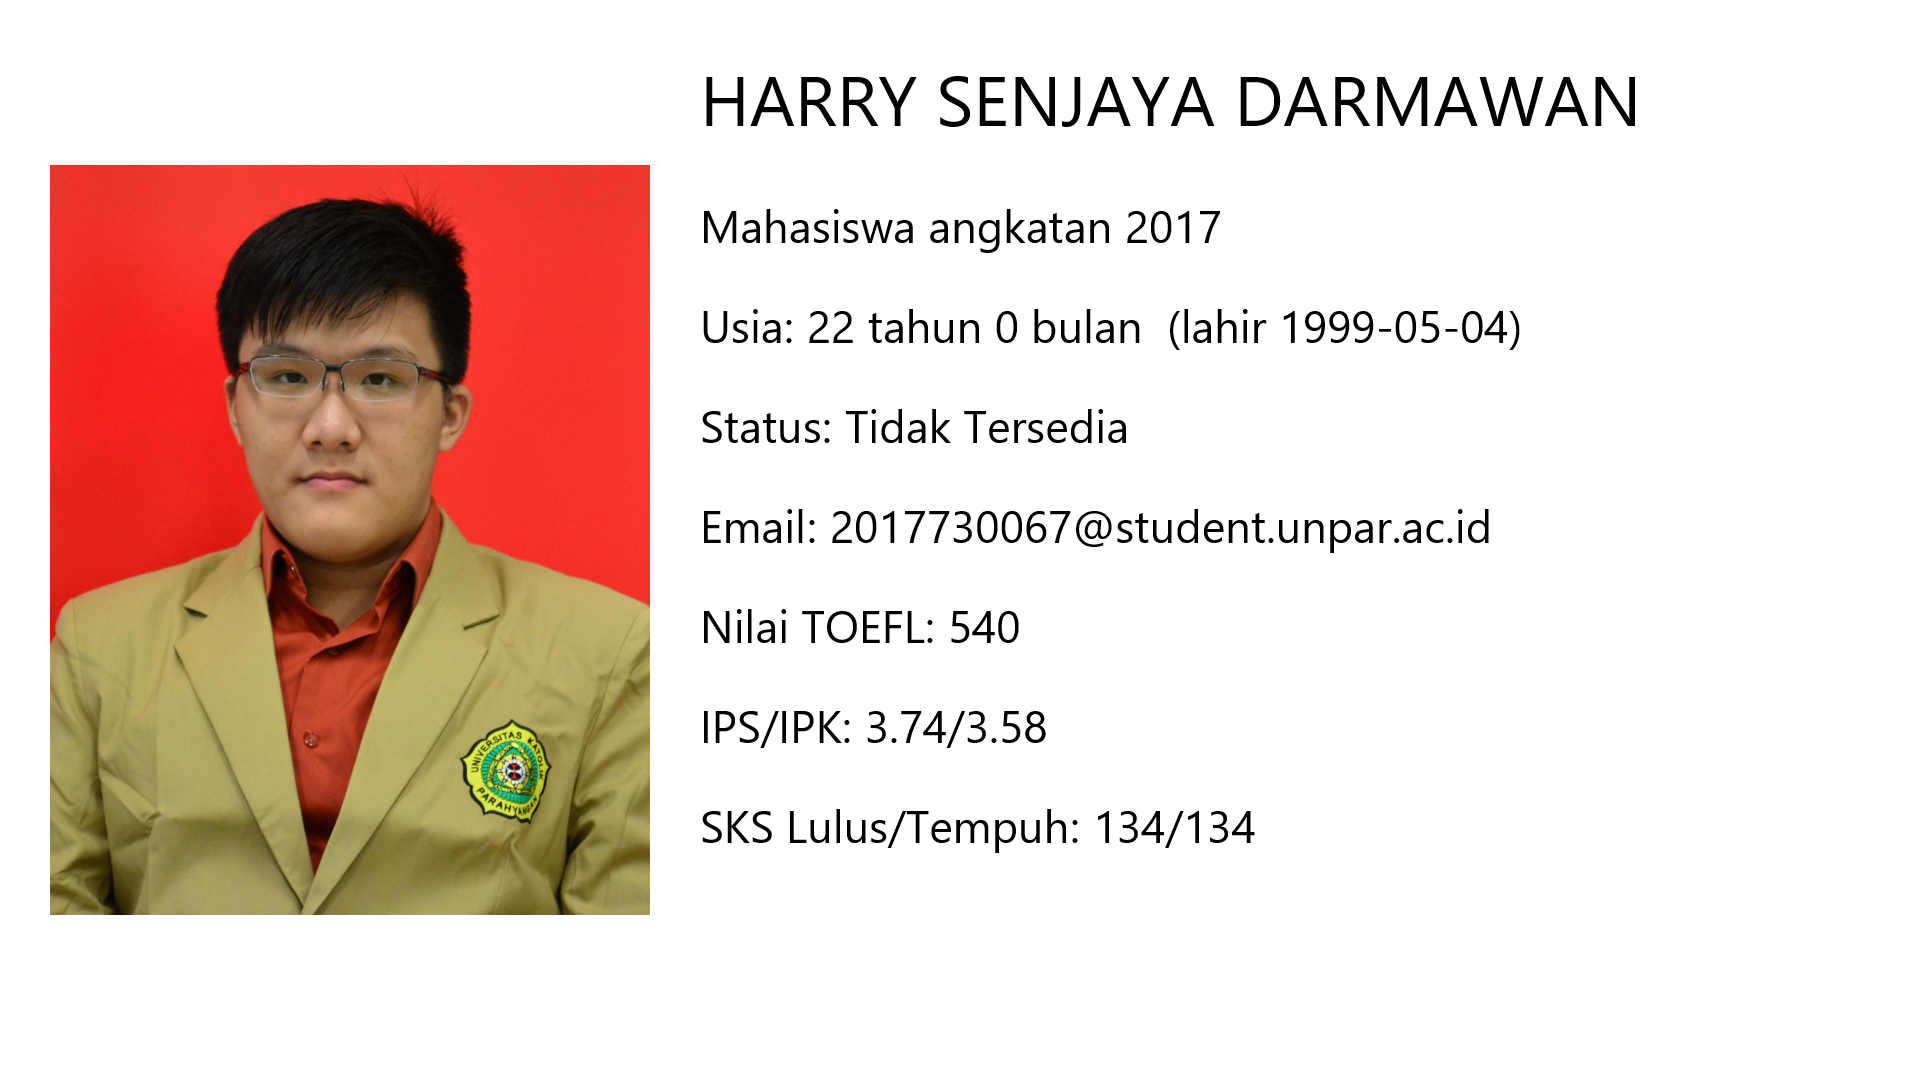
\includegraphics[scale=0.3]{Gambar/hasil.png}
	\caption{Tampilan \textit{Screensaver}}
	\label{fig:5_hasil}
\end{figure}